\section{Overview}
% -- TODO --


\section{Component View}
% -- TODO --

\subsection{Database}
The application database will be managed using a Relational DBMS.
It allows the reading of data, ensuring users the ability to log in and access the applications of interest and check the stored data.
It is also used for data manipulation (insertion, modification and deletion).
The use of a Relational DBMS guarantees the fundamental properties for a database of this type:
\begin{itemize}
  \item \textit{Atomicity}: no partial executions of operations.
  \item \textit{Consistency}: the database is always in a consistent state.
  \item \textit{Isolation}: each transaction is executed in an isolated and independent way.
  \item \textit{Durability / Persistence}: changes made are not lost.
\end{itemize}
The database will offer to the Application Server an interface that it can use to interact with the database.
The data stored in the database must be considered personal and confidential, therefore, procedures must be implemented to safeguard the stored information.\\
Particular attention must be paid to the reading permissions granted to users and to the encryption of passwords used to access the services offered.
Below is the designed E-R diagram:

\begin{figure}[H]
  \begin{center}
  	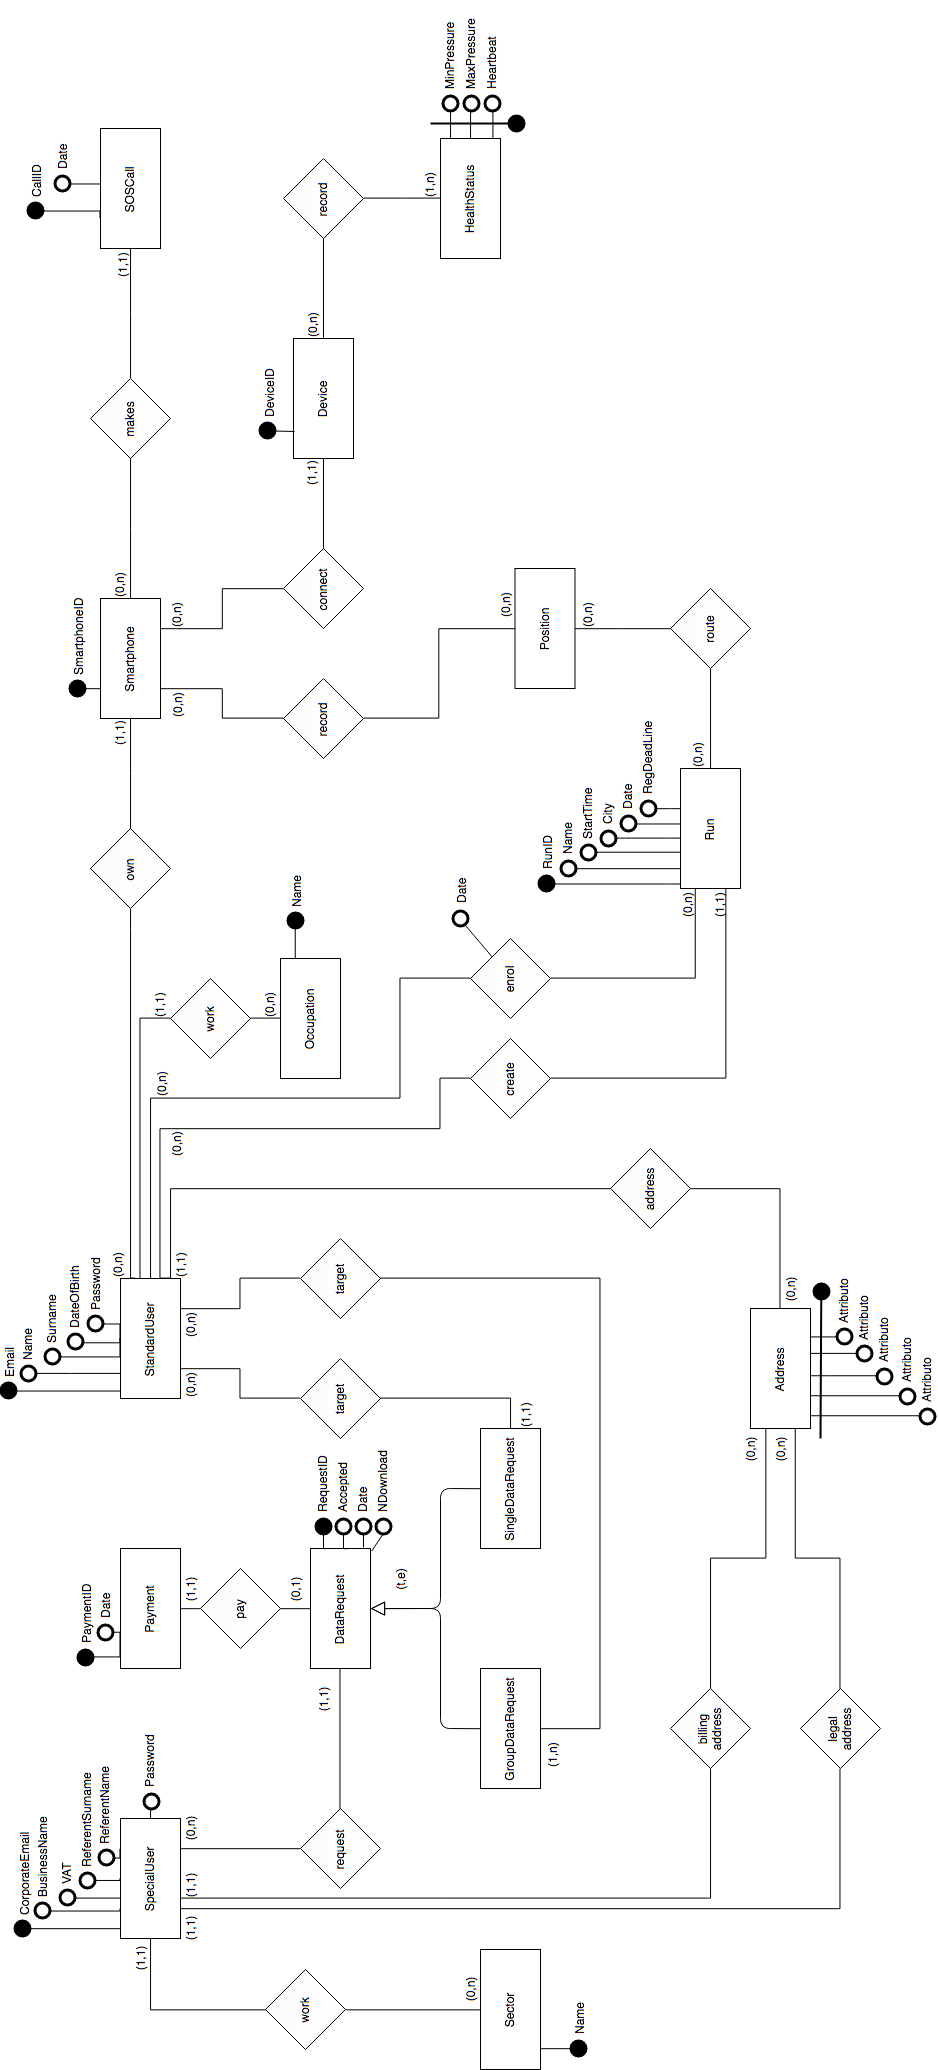
\includegraphics[height=0.68\paperheight]{./img/ER.png}
    \hspace{0.05\linewidth}
    \centering
    \caption{\textit{E-R} Diagram.}
		\label{img:ER_Diagram}
    \end{center}
\end{figure}

\subsection{Application Server}
This is the crucial layer of the system to be. The main feature of the \textit{Application Server} is to describe rules and work-flows of all the functionalities provided by the application.\\
The \textit{Application Server} must have intefaces to communicate with the \textit{Web Server} and the \textit{Mobile Apps}, it has also to communicate through interfaces with all the \textit{External Services} (Maps Service, SOS Service and Payment Service).\\
Moreover, the \textit{Application Server} is the only entity of the system that is granted to communicate with the DBMS.
Following this brief introduction there are the logic modules and their descriptions.

\paragraph{Server Access Point}
This module provides the access point to the \textit{Application Server} for the \textit{Web Server} and the \textit{Mobile Apps}. It routes different users in the correct \textit{User Manger} module.

\begin{figure}[H]
  \begin{center}
  	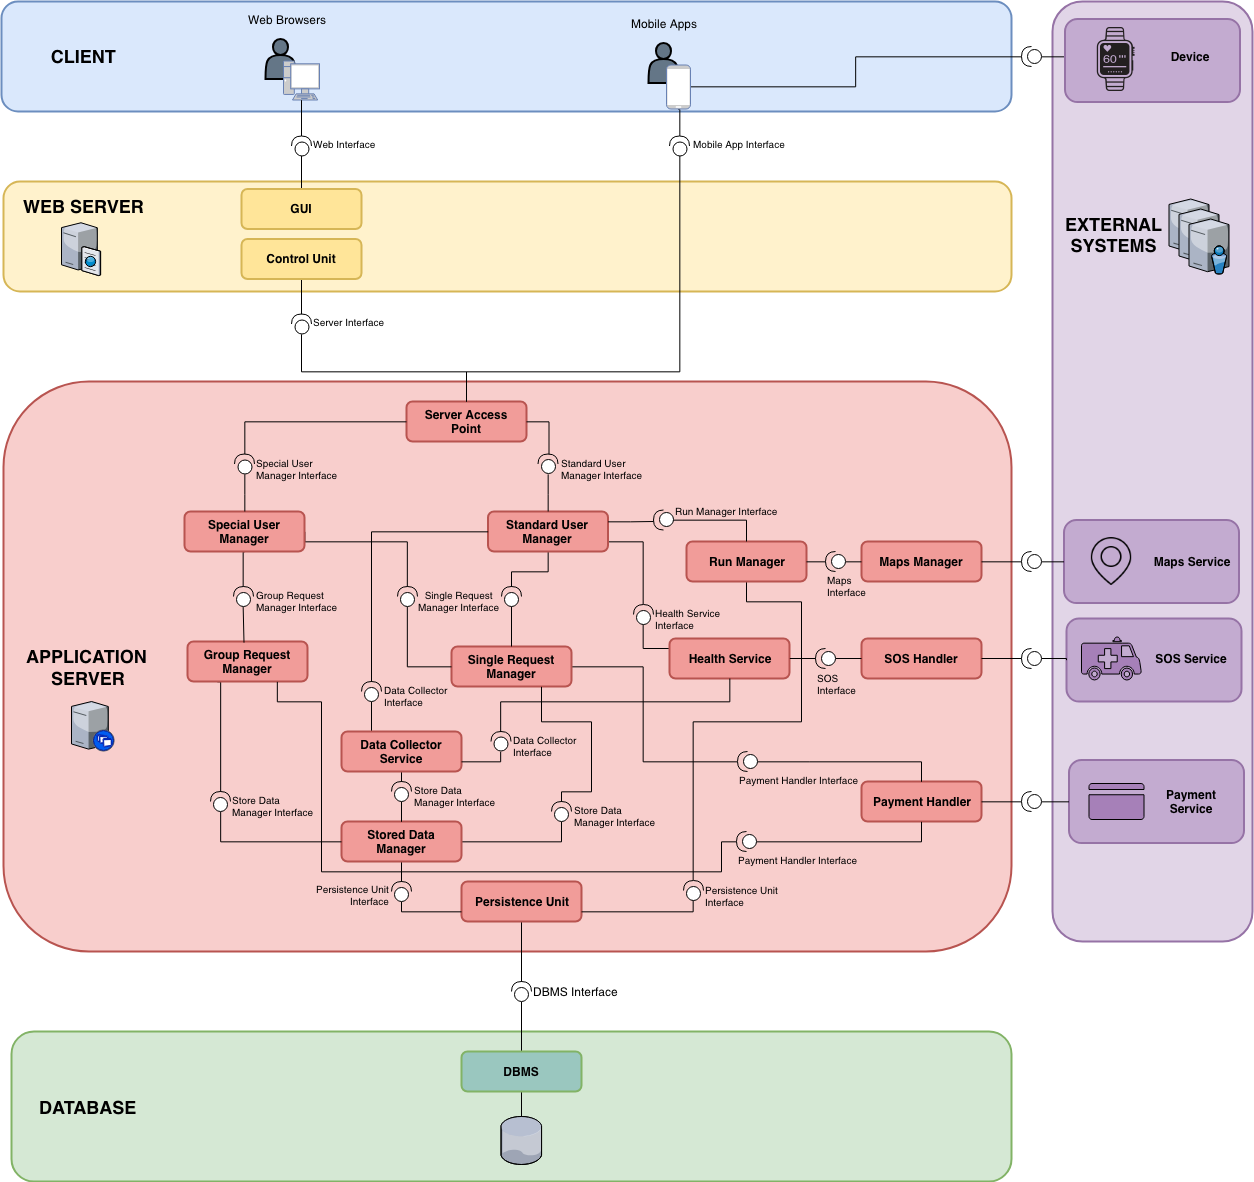
\includegraphics[width=\textwidth]{./img/GlobalComponent.png}
    \hspace{0.05\linewidth}
    \centering
    \caption{\textit{Global Component} Diagram.}
		\label{img:GlobalComponent}
    \end{center}
\end{figure}
\section{Deployment View}

\section{Runtime View}

\section{Component Interfaces}

\section{Selected Architectural Styles and Patterns}

\section{Other Design Decisions}
